% Statistics and Computing submission — adapted from Springer Nature sn-jnl class
\documentclass[pdflatex,sn-mathphys-ay]{sn-jnl}% Author-Year Reference Style

\usepackage{graphicx}%
\usepackage{multirow}%
\usepackage{amsmath,amssymb,amsfonts}%
\usepackage{amsthm}%
\usepackage{mathrsfs}%
\usepackage[title]{appendix}%
\usepackage{xcolor}%
\usepackage{textcomp}%
\usepackage{manyfoot}%
\usepackage{booktabs}%
\usepackage{algorithm}%
\usepackage{algorithmicx}%
\usepackage{algpseudocode}%
\usepackage{listings}%
%%%%

\theoremstyle{thmstyleone}%
\newtheorem{theorem}{Theorem}%
\newtheorem{proposition}[theorem]{Proposition}%

\theoremstyle{thmstyletwo}%
\newtheorem{example}{Example}%
\newtheorem{remark}{Remark}%

\theoremstyle{thmstylethree}%
\newtheorem{definition}{Definition}%

\raggedbottom

\begin{document}

\title[On the Alignment Between Marginal Uncertainty Measures and Conditional Decision Risk]{On the Alignment Between Marginal Uncertainty Measures and Conditional Decision Risk in Estimator Selection}

\author*[1]{\fnm{Y.} \sur{Wang}}\email{yw1580@scarletmail.rutgers.edu}

\affil*[1]{\orgdiv{Department of Statistics}, \orgname{Rutgers University}, \orgaddress{\city{Piscataway}, \state{NJ}, \country{USA}}}

\abstract{Conformal prediction provides distribution-free uncertainty quantification for any estimator, but whether these uncertainty signals can guide estimator selection under nonlinear heterogeneity is not well understood. We study whether marginal residual-based uncertainty summaries can support estimator selection when the decision target is conditional prediction risk. We prove that, under heterogeneous bias geometry, no selector based solely on marginal absolute-residual functionals can be uniformly decision-consistent: if two estimators induce identical marginal distributions of absolute residuals but their conditional risk surfaces cross over the covariate space, then any such selector must incur a non-vanishing misalignment probability. We also identify a positive boundary: under a common symmetric noise family and uniformly ordered absolute bias, residual-quantile rankings preserve the conditional risk ordering. Simulations across six data-generating regimes and seven estimators show that the empirical behavior of conformal width and related surrogates is consistent with this boundary, and that aggregation-based corrections inherit the same limitation.}

\keywords{Conformal prediction, Model selection, Uncertainty quantification, Decision theory, Bias crossing, Misalignment probability}

\maketitle

%% ===== Declarations =====
\section*{Declarations}
\textbf{Funding:} No funding was received to assist with the preparation of this manuscript.
\textbf{Competing interests:} The author has no relevant financial or non-financial interests to disclose.
\textbf{Author contributions:} Y. Wang conceived the study, designed and implemented the experiments, analyzed the results, and wrote the manuscript.
\textbf{Data availability:} The simulation code and experimental configurations are available at \url{https://github.com/wyp629929/estimator-selection-nl}. The real datasets used in this study are publicly available: Home Credit Default Risk (Kaggle), PIMA Diabetes (UCI), and Superconductivity (UCI).

%% ============================================================
\section{Introduction}
\label{sec:intro}
% ============================================================

Estimator selection is a recurring challenge in applied statistics. When the data-generating process is unknown, practitioners must choose among classical methods (ordinary least squares, ridge, lasso), tree-based ensembles (random forests, gradient boosting), and deep learning estimators without clear guidance on which will perform best. Conformal prediction \citep[CP;][]{angelopoulos2023} is an increasingly popular framework for uncertainty quantification that provides finite-sample valid prediction intervals under exchangeability, and its signals, particularly interval width, are naturally attractive as candidates for guiding estimator choice. In practice, narrower prediction intervals are frequently interpreted as evidence of superior predictive performance, and several recent works have proposed using CP-based criteria for model or configuration selection \citep{yang2024conformal}. These practices implicitly treat CP uncertainty as informative about relative model quality.

Whether CP signals can inform selection decisions depends on an assumption that has received limited systematic evaluation. The assumption is that the uncertainty ranking induced by CP aligns with the ranking induced by actual prediction risk, particularly under nonlinear heterogeneity and across diverse estimator classes. This assumption is not trivial: CP width is a marginal absolute-residual quantile functional, while decision-optimal selection requires conditional squared-risk comparisons. These two functionals operate on different scales (absolute versus squared), at different levels of aggregation (marginal versus conditional), and their alignment requires restrictive conditions on estimator bias structure. The misalignment is not specific to conformal prediction. Selection rules based on residual-based marginal functionals (defined formally in Section~\ref{sec:boundary} as any permutation-invariant function of absolute residuals) face the same structural barrier under heterogeneous bias, because the reduction from conditional function to marginal scalar is lossy with respect to pointwise decision ordering. CP provides a particularly clean testbed for studying this question because its finite-sample validity guarantees remove coverage-driven confounders, isolating the functional alignment problem. We emphasize that our results concern a specific class of selectors based on marginal absolute-residual summaries; they do not rule out other approaches to estimator selection such as conditional risk estimation, Bayesian model averaging, or directly decision-aware procedures.

\paragraph{This paper.}
We study whether CP-based uncertainty signals induce rankings that are consistent with decision-optimal estimator selection under heterogeneous nonlinearity, where decision-optimal selection is defined with respect to conditional prediction risk under each data-generating process. Using controlled simulations across six data-generating processes (linear, mildly nonlinear, smooth nonlinear, threshold, high-dimensional sparse, and heteroscedastic) with seven estimators (ordinary least squares, ridge regression, lasso, random forest, XGBoost, LightGBM, and a deep neural network), we compare two CP signals (split-conformal interval width and conformalized regret bounds) against an oracle decision standard defined by conditional prediction risk.

\paragraph{Main finding.}
We find that marginal uncertainty functionals, whether CP interval width or per-point regret bounds, systematically misalign with decision-optimal estimator ordering under heterogeneous bias. The root cause is a persistent gap between the marginal residual scale that CP measures and the pointwise bias--variance decomposition that optimal selection requires. Alignment is strongest when a single estimator dominates, as in the high-dimensional regime where lasso's clear advantage keeps $\Delta$ at 0.345. In contrast, competitive settings with heterogeneous estimator biases, such as the linear regime where tree-based and neural network models introduce non-negligible approximation bias even for linear targets, yield higher misalignment ($\Delta = 0.600$). Outside this boundary, the functional gap is systematic and was not circumvented by the aggregation methods studied here.

\paragraph{Contributions.}
Our contribution is threefold. First, we formalize the ranking--decision gap by separating marginal residual functionals from conditional decision risk and establish an impossibility result for pointwise decision recovery under bias crossing. Second, we prove a sufficient alignment condition under uniformly ordered absolute bias and common symmetric noise, which clarifies when marginal uncertainty summaries can remain decision-relevant. Third, we show through controlled simulations and repeated-split real-data diagnostics that conformal width, localized regret surrogates, and related residual summaries behave in accordance with this boundary rather than failing for purely implementation-specific reasons. Real-data validation across three public datasets is consistent with this pattern. We emphasize that our findings pertain to the CP signal constructions and model classes considered in this study.

\paragraph{Organization.}
Section~\ref{sec:prelim} reviews background on the estimators and conformal prediction. Section~\ref{sec:design} describes the experimental framework and formalizes the ranking--decision framework. Section~\ref{sec:results} presents the main empirical findings, the boundary condition for equivalence, aggregation consequences, and real-data robustness. Section~\ref{sec:conclusion} concludes.

% ============================================================
\section{Preliminaries and Related Work}
\label{sec:prelim}
% ============================================================

\subsection{Classical and Machine Learning Estimators}

Consider the standard regression setting $y = f(X) + \varepsilon$ with $\mathbb{E}[\varepsilon] = 0$ and $\mathbb{V}[\varepsilon] = \sigma^2$. Classical linear estimators, including ordinary least squares (OLS), ridge regression, and lasso \citep{tibshirani1996}, offer consistency and tractable inference under correct specification but degrade under nonlinearity \citep{lehmann2006}.

Tree-based ensemble methods construct prediction functions through recursive partitioning. Random forests \citep[RF;][]{breiman2001} average $B$ trees trained on bootstrap samples; gradient boosting methods \citep{chen2016, ke2017} build additive ensembles sequentially. Deep neural networks (DNNs) approximate the regression function through compositional layers with nonlinear activations \citep{goodfellow2016}.

These methods are reviewed briefly in Section~\ref{sec:methods}; for a discussion of their statistical properties, see \citet{scornet2015}, \citet{mentch2016}, and \citet{farrell2021}.

\subsection{Conformal Prediction}

Split conformal prediction \citep{lei2018, angelopoulos2023} provides finite-sample valid prediction intervals under exchangeability. Given a training set of size $n$ and a held-out calibration set of size $n_{\text{cal}}$, the split CP prediction interval at a new point $X_{\text{new}}$ for estimator $\hat{f}_M$ is
\begin{equation}
    \hat{f}_M(X_{\text{new}}) \pm q_M,
    \label{eq:split-cp}
\end{equation}
where $q_M$ is the $\lceil (n_{\text{cal}}+1)(1-\alpha)\rceil / n_{\text{cal}}$ quantile of calibration absolute residuals $|Y_i - \hat{f}_M(X_i)|$.

The interval width $2q_M$ is constant for all test points and reflects the estimator's marginal predictive uncertainty. Refinements include locally adaptive (normalized) CP, where residuals are scaled by a fitted dispersion model $\hat{\sigma}(X)$ to produce per-point widths $2q \cdot \hat{\sigma}(X_{\text{new}})$. See \citet{lei2018, angelopoulos2023} for a review of these variants.

\subsection{Related Work: Conformal Prediction for Model Selection}

A growing body of work uses CP for model or configuration selection. \citet{yang2024conformal} establish oracle inequalities for selecting among candidate models to minimize prediction set width while maintaining coverage validity. Their focus is on validity guarantees of conformal-based selection; they show that an oracle inequality holds under certain conditions, ensuring that the selected model's coverage is controlled at a target level.

The present paper addresses a distinct question. Rather than asking whether CP-based selection maintains validity (coverage), we ask whether CP-based \textit{ranking functionals} align with \textit{decision-optimal ordering} defined by conditional prediction risk. This distinction, validity versus decision optimality, is the central axis of our investigation. A CP-based selection may maintain nominal coverage while systematically picking risk-suboptimal models, and it is this possibility we examine.

Several related lines of work address aspects of this question. \citet{liang2024conformal} observe that selecting models to minimize CP width is not aligned with minimizing prediction error (e.g., MSE), noting that these two criteria serve distinct objectives. However, their focus is on validity guarantees after model selection rather than on systematically characterizing the alignment gap itself. \citet{bao2025optimal} explicitly note that minimizing the width is not directly relevant to the risk of downstream decision and propose CROiMS, a procedure that selects models according to conditional decision risk at each test point. Their CROiMS framework is closely related to our local oracle $M^*(x)$; however, they operate within a robust optimization setting and propose a constructive selection rule, whereas our contribution is diagnostic---we prove an impossibility result for marginal residual selectors and empirically delineate the conditions under which alignment fails. \citet{romano2019conformalized} develop conformalized quantile regression, which produces per-point adaptive intervals that can yield different rankings than marginal split CP. \citet{rosenfeld2022riskoptimal} study constructing prediction sets that are optimal with respect to a given decision task rather than merely valid. \citet{jin2023model} directly address model selection within the conformal framework. \citet{barber2021limits} establish fundamental limits on distribution-free conditional inference, formalizing the gap between marginal and conditional quantities that the present paper examines in the estimator selection context. From a decision-theoretic perspective, the problem can be framed using the theory of proper scoring rules~\citep{gneiting2007strictly}. The squared-error loss is a proper scoring rule for the conditional mean, and our findings show that CP interval width, which is not a scoring rule, does not preserve its ordering under heterogeneous bias. Related work on CP for aggregation and decision-aware uncertainty quantification addresses partially overlapping questions but from the perspective of improving decisions rather than diagnosing the alignment between CP signals and decision targets. Our contribution is diagnostic: we show that under nonlinear heterogeneity, the mismatch between CP-based ranking and decision-optimal selection is persistent across the settings we examine and is not merely a matter of tuning or calibration. The key distinction between our work and these prior studies is that we provide the first formal impossibility result (Proposition~2) establishing that no marginal residual selector can achieve uniform decision consistency under bias crossing, together with a systematic empirical characterization across six regimes, seven estimators, and multiple CP variants.

% ============================================================
\section{Experimental Design}
\label{sec:design}
% ============================================================

\subsection{Simulation Framework}

We consider six data-generating processes (DGPs), each following
\begin{equation}
    y = f(X) + \varepsilon,
\end{equation}
with $X_j \stackrel{\text{i.i.d.}}{\sim} N(0,1)$ for $j=1,\ldots,p$, $\varepsilon \sim N(0,1)$, and $n = 500$ observations per replication. We use $B = 500$ replications for baseline performance estimation and $B = 200$ for ranking--decision experiments (the latter requires nested calibration that is computationally more intensive). The six DGPs are designed to span distinct nonlinearity regimes encountered in applied work:

\begin{enumerate}
    \item \textbf{Linear} ($p=10$). The regression function is $f(X) = X\beta$ with $\beta = (2,\allowbreak -1.5,\allowbreak 0.8,\allowbreak 0.5,\allowbreak -0.3,\allowbreak 0,\allowbreak \ldots,\allowbreak 0)^\top$, providing a baseline where classical linear methods are optimally specified.

    \item \textbf{Mildly nonlinear} ($p=10$). The function is $f(X) = X\beta + 0.3\sin(X_1)$, adding a mild nonlinear perturbation to the linear specification. This DGP provides an intermediate gradient between the linear and fully nonlinear regimes.

    \item \textbf{Nonlinear (smooth compositional)} ($p=10$). The function is $f(X) = \sin X_1 + \log(1 + |X_2|) + X_3X_4$, a smooth additive function with pairwise interactions. This structure favors ReLU networks, which approximate compositional functions efficiently through hierarchical representations~\citep{schmidt2020}.

    \item \textbf{Threshold} ($p=10$). The function $f(X) = 2 \cdot \mathbf{1}(X_1 > 0) + \log(1 + |X_2|) \cdot \mathbf{1}(X_3 > 0) - 1$ introduces discrete discontinuities and threshold effects. This DGP is designed to favor tree-based methods, whose recursive partitioning naturally captures piecewise constant structures.

    \item \textbf{Moderately high-dimensional sparse} ($p=100$). The linear model has $s = 5$ non-zero coefficients, $\beta = (2,\allowbreak -1.5,\allowbreak 0.8,\allowbreak 0.5,\allowbreak -0.3,\allowbreak 0,\allowbreak \ldots,\allowbreak 0)^\top$. With $n=500$, the ratio $p/n = 0.2$ is moderate rather than ultra-high-dimensional; we use the term high-dimensional as shorthand but note that more extreme ratios may produce different alignment patterns.

    \item \textbf{Heteroscedastic} ($p=10$). The mean function is the same linear specification as DGP 1, but the noise is heteroscedastic: $\varepsilon \sim N(0, \sigma^2(X))$ with $\sigma(X) = 0.5 + 0.5|X_1|$. This DGP tests whether CP-based alignment degrades under variance heterogeneity, in a setting where the linear mean function gives estimators approximately similar bias structure.
\end{enumerate}

\subsection{Methods and Implementation}
\label{sec:methods}

Seven estimators are compared across all scenarios. Classical baselines include ordinary least squares (OLS), ridge regression (regularization parameter $\lambda = 1$), and lasso (fixed regularization parameter $\alpha = 0.01$). Tree ensemble methods include random forest (200 trees, max depth 10, min samples leaf 5), XGBoost~\citep{chen2016} (200 trees, max depth 6, learning rate 0.1), and LightGBM~\citep{ke2017} (200 trees, max depth 6, learning rate 0.1). The deep neural network (DNN) has three hidden layers (128-64-32 units) with ReLU activations, dropout (0.2), and is trained with the Adam optimizer for up to 200 epochs with early stopping (patience 20) on a 20\% validation split. For DNN training, features are standardized using training-set means and standard deviations.

All analyses use Python 3.13 with scikit-learn 1.6, XGBoost 2.1, LightGBM 4.5, and PyTorch 2.5, running on Apple M4 Pro with 32 GB memory. Monte Carlo replications use independent seeds $(2024 + \text{rep})$ for full reproducibility.

\subsection{Conformal Prediction Signals}
\label{sec:cp-signals}

We construct two CP-based ranking signals for each estimator $M$. All are instances of a general ranking functional $R(M) = \phi(\hat{Z}_M)$, where $\hat{Z}_M$ is a conformal uncertainty estimate.

\paragraph{Signal 1: Split-CP interval width.} For each estimator $M$, we compute the standard split-conformal prediction interval~\citep{lei2018, angelopoulos2023} using a held-out calibration set. The absolute residuals on the calibration set are $|Y_i - \hat{f}_M(X_i)|$, and the conformal quantile is
\begin{equation}
    q_M = Q_{1-\alpha}\bigl(|Y_{\text{cal}} - \hat{f}_M(X_{\text{cal}})|\bigr),
\end{equation}
where $Q_{1-\alpha}$ denotes the $\lceil (n_{\text{cal}}+1)(1-\alpha)\rceil / n_{\text{cal}}$ empirical quantile. The interval width $2q_M$ is constant for all test points and serves as the simplest CP-based ranking signal.

\paragraph{Signal 2: Conformalized regret bound $U_M$.}
The regret-based signal $U_M(x)$ quantifies excess loss relative to the best estimator, rather than absolute prediction uncertainty. We define the excess loss of estimator $M$ at point $x$ as $R_M(x) = \ell(\hat{f}_M(x), y) - \min_{M'} \ell(\hat{f}_{M'}(x), y)$, where $\ell$ is squared error. We fit models $\hat{r}_M(x)$ and $\hat{a}_M(x)$ for the conditional mean and dispersion of $R_M$ using random forests on a meta-training set. A joint conformal quantile $q$ is then calibrated on a separate meta-calibration set via the max-normalized scores
\begin{equation}
    s_i = \max_{M \in \mathcal{M}} \frac{R_M(X_i) - \hat{r}_M(X_i)}{\hat{a}_M(X_i)}.
\end{equation}
The regret bound is $U_M(x) = \max\{0,\ \hat{r}_M(x) + q \cdot \hat{a}_M(x)\}$. By construction, $P(R_M(X) \leq U_M(X) \ \forall M \in \mathcal{M}) \geq 1-\alpha$ marginally.

\subsection{Ranking--Decision Framework}
\label{sec:framework}

Let $\mathcal{M} = \{M_1, \ldots, M_m\}$ be the set of $m = 7$ candidate estimators. For a fixed DGP and test point $x$, we compare two functionals:

\begin{itemize}
    \item \textbf{Ranking functional} $R(M)$: a scalar summary of CP-based uncertainty for estimator $M$. We consider the two signals defined in Section~\ref{sec:cp-signals}: the split-CP width $2q_M$ (constant per replication) and the conformalized regret bound $U_M(x)$.
    \item \textbf{Decision functional} $D(M)$: the conditional prediction risk,
    \begin{equation}
        D(M) = \mathbb{E}\bigl[(f_0(X) - \hat{f}_M(X))^2 \mid X\bigr] = (f_0(X) - \mathbb{E}[\hat{f}_M(X)])^2 + \mathbb{V}(\hat{f}_M(X)),
    \end{equation}
    where $f_0$ is the true regression function. This quantity represents the oracle benchmark for estimator comparison and is computable in simulation because $f_0$ is known.
\end{itemize}

Because the decision functional is conditional on $X$, the optimal estimator can vary across the predictor space. We therefore distinguish two oracle targets and evaluate each functional against its corresponding oracle only. The \textbf{global oracle} $M^\ast_{\text{global}} = \arg\min_M \mathbb{E}[D(M|X)]$ selects the estimator with smallest average risk, appropriate for evaluating global selection criteria (CP interval width). The \textbf{local oracle} $M^\ast(x) = \arg\min_M D(M|x)$ selects per point, appropriate for evaluating per-point signals ($U_M$). We evaluate each at its intended decision level, and the two settings are not mixed in evaluation.

The primary diagnostic is the misalignment probability
\begin{equation}
    \Delta = \mathbb{E}_{\text{DGP}}\bigl[\,\mathbf{1}\{\arg\min_{M} R(M) \neq \arg\min_{M} D(M)\}\bigr],
    \label{eq:delta}
\end{equation}
where the expectation is over repeated finite-sample draws from the fixed DGP. The uniform random baseline $1 - 1/m$ serves as a mathematical reference under equiprobable model selection. In practice, estimator performance is structured, so this baseline is a conservative upper bound on the misalignment of any informed selection rule.

Supporting diagnostics include pairwise ranking accuracy (the proportion of model pairs $(M_i, M_j)$ for which $R(M_i) < R(M_j)$ agrees with $D(M_i) < D(M_j)$, baseline 0.5) and top-$k$ coverage (the proportion of test points for which the set of $k$ models with smallest $R$ contains the conditionally optimal model).

These diagnostics distinguish between two tasks: \textit{model ranking} (ordering estimators by quality, measured by pairwise accuracy) and \textit{decision policy} (selecting a single estimator per point, measured by $\Delta$ and top-$k$ coverage). Pairwise ranking accuracy can be high even when argmin selection fails, a pattern we observe for $U_M$, because consistent ordering of estimator pairs does not guarantee correct identification of the optimal estimator in the tail of the ordering.

For the ranking--decision experiments, each replication uses a five-way data split: 50\% for training, 15\% for meta-fitting (regret model estimation), 10\% for meta-calibration (joint conformal quantile), 10\% for final calibration (CRGA re-conformalization), and 15\% for testing. For models requiring hyperparameter tuning (DNN), an additional 20\% hold-out from the training set is used for early stopping.

\subsection{Real Data}
\label{sec:real-data-design}

Three publicly available datasets are used to assess whether the alignment pattern observed in simulation extends to unknown, non-simulated DGPs: Home Credit Default Risk (307,511 observations, 66 numerical features), PIMA Diabetes (768, 8), and Superconductivity (21,263, 81). For each dataset, we compute $\hat{\Delta}$ across multiple random train-test splits (70\% training, 30\% test). Unlike the simulation setting where $f_0$ is known and $D(M)$ is the conditional prediction risk, for real data we define $\hat{D}(M)$ as the test-set MSE, which serves as an observable proxy. The real-data analysis should therefore be interpreted as a robustness check rather than a direct validation of the simulation metric. We emphasize that these experiments are not intended for model comparison or benchmark ranking.

For classification datasets (PIMA, Home Credit), we use test MSE as the observable proxy for prediction risk, noting that this is a marginal metric and therefore the comparison evaluates agreement between two marginal summary measures rather than providing a direct test of the simulation-based claims about conditional risk. We flag this as a limitation of the real-data validation and discuss implications in Section~\ref{sec:real-data}.

\subsection*{Robustness to Modeling and Evaluation Concerns}

This section clarifies the scope, interpretation, and structural assumptions underlying our results, to ensure that the empirical and theoretical findings are interpreted within the appropriate class of decision problems and functional representations.

\paragraph{1. Scope of marginal uncertainty functionals.}
We study marginal residual functionals that map predictive errors to scalar summaries of uncertainty, using conformal prediction as a representative and well-defined instance of this broader class.

\paragraph{2. Interpretation of simulation evidence.}
The simulation design is intended to illustrate regime-dependent behavior consistent with the proposed structural mechanism, rather than to provide benchmark comparisons of predictive performance. Accordingly, the reported misalignment patterns should be interpreted as qualitative regime identification rather than quantitative performance evaluation.

\paragraph{3. Structural mechanism and generality.}
The bias-crossing condition introduced in Proposition~2 provides a transparent sufficient condition for misalignment between marginal and conditional decision functionals. More generally, the same phenomenon arises whenever the estimator class exhibits spatially heterogeneous or non-monotone bias structure over the covariate space. The purpose of the crossing example is therefore illustrative rather than exhaustive.

\paragraph{4. Effect of alternative conformal constructions.}
Local and normalized conformal procedures modify the scale of residuals but preserve the fundamental reduction of conditional structure into marginal summaries. As a consequence, improvements in calibration may not in general translate into improved alignment with conditional decision functionals. To test this directly, we implemented conformalized quantile regression (CQR; Romano et al., 2019) as an alternative CP signal that produces per-point adaptive intervals via quantile regression. Across all six regimes, CQR-based selection achieved $\Delta_{\text{CQR}}$ between 0.855 and 1.000, uniformly worse than split CP width and validation-MSE baselines. In three regimes it was indistinguishable from always picking the wrong model ($\Delta = 1.000$). The poor performance reflects the difficulty of estimating conditional quantiles from limited data ($n=250$ for quantile regression training), which compounds the underlying alignment gap rather than resolving it. We caution that this result may depend on the specific quantile regression implementation (gradient boosting with 200 trees). Alternative methods such as quantile random forests or neural-network-based quantile regression could yield different alignment behavior, though we expect the finite-sample estimation challenge to persist.

We further tested CV+ (cross-validation plus) prediction intervals, which use 5-fold cross-validated residuals to construct per-point intervals. CV+ achieves $\Delta_{\text{CV+}}$ between 0.043 and 0.834 across the six regimes. It performs well in regimes where one estimator dominates (high-dimensional: $\Delta_{\text{CV+}} = 0.043$; threshold: $0.123$) but struggles under strong nonlinearity (nonlinear: $\Delta_{\text{CV+}} = 0.834$), where estimator stability across folds degrades. This pattern confirms that the alignment gap is not an artifact of any single CP construction. It persists across split CP, normalized CP, CQR, and CV+, and is instead a consequence of the marginal-to-conditional functional mismatch that no residual-based summary fully escapes.

\paragraph{5. Interpretation of localized surrogate functionals.}
The per-point regret functional $U_M(x)$ is introduced as a conformalized diagnostic tool for probing local structure in predictive uncertainty. It is not intended as an optimal estimator of conditional risk. Its performance should therefore be interpreted as reflecting the inherent difficulty of recovering conditional risk ordering from smoothed residual representations, rather than as a limitation of a specific modeling choice.

\paragraph{6. Evaluation framework consistency.}
We distinguish between global and local decision problems. Global CP-based rankings are evaluated against a global oracle selecting a single estimator per dataset, whereas per-point regret-based rankings are evaluated against a local oracle defined pointwise in the covariate space. These two decision regimes correspond to different information structures and are not combined within a single evaluation criterion.

% ============================================================
\section{Results: Characterizing the Alignment Boundary}
\label{sec:results}
% ============================================================

\subsection{Formalism Recap}

We evaluate the alignment between CP-based ranking functionals $R(M)$ and the decision-optimal functional $D(M)$ across six DGPs and seven estimators. The primary diagnostic is the misalignment probability $\Delta$ (\ref{eq:delta}), supplemented by pairwise ranking accuracy and top-$k$ coverage. All CP signals are evaluated on held-out test sets (30\% of $n=500$). The simulations are designed to validate the predicted regime structure of Propositions~1--2 rather than to estimate finite-sample performance; we focus on whether the observed $\Delta$ patterns conform to the bias-crossing mechanism rather than on their precise magnitudes.

We report the baseline MSE performance across all regimes in Table~\ref{tab:baseline}.

\begin{table}[t]
    \centering
    \caption{Mean squared error (MSE) across six simulation regimes. All regimes use $B=500$ replications, except heteroscedastic and mildly nonlinear which use $B=200$ due to the additional computational cost of the nested calibration design required for the ranking--decision experiments involving these regimes.}
    \label{tab:baseline}
    \begin{tabular}{lcccccc}
        \toprule
        Method & Linear & Mild nonlin. & Nonlinear & Threshold & High-dim & Heterosc. \\
        \midrule
        OLS     & 1.03 & 1.04 & 2.27 & 1.49 & 1.42 & 0.97 \\
        Ridge   & 1.03 & 1.04 & 2.27 & 1.49 & 1.41 & 0.97 \\
        Lasso   & 1.03 & 1.04 & 2.26 & 1.48 & 1.27 & 0.97 \\
        RF      & 1.90 & 2.07 & 1.98 & 1.13 & 2.32 & 2.01 \\
        XGBoost & 1.85 & 2.07 & 1.95 & 1.30 & 2.28 & 1.96 \\
        LightGBM& 1.68 & 1.82 & 1.74 & 1.32 & 1.82 & 1.76 \\
        DNN     & 1.23 & 1.30 & 1.50 & 1.47 & 2.61 & 1.23 \\
        \bottomrule
    \end{tabular}
\end{table}

\subsection{Main Result: Non-Equivalence Under Nonlinearity}

Table~\ref{tab:misalignment} reports the primary diagnostic $\Delta$ and supporting metrics across all six regimes, using $B = 200$ replications with the five-way data split described in Section~\ref{sec:framework}. The table distinguishes between global model selection (CP interval width, which is constant per estimator per replication) and per-point selection (the regret bound $U_M$, which varies across test points). Several patterns emerge.

\paragraph{Per-point selection is weakly informative.} For the regret bound $U_M$, the misalignment probability $\Delta$ ranges from 0.713 to 0.786 across all regimes, only modestly below the random baseline of 0.857. This means that per-point CP-based model selection offers limited information: knowing which estimator has the narrowest CP interval at a given test point provides only a small advantage over random choice. Notably, while $U_M$ exhibits markedly smaller variance than the global CP width (Figure~\ref{fig:gap-vs-regime}), this variance reduction reflects the conformalized regret construction rather than improved decision relevance: $U_M$'s mean $\Delta$ remains close to the random baseline across all regimes, indicating that its precision does not translate into more accurate selection. The top-2 coverage of $U_M$, the probability that the conditionally optimal model is among the two estimators with smallest $U_M$, ranges from 0.358 to 0.470, above the random baseline of 0.286 but far from reliable.

\paragraph{Ranking improvement does not translate to selection.}
The conformalized regret bound $U_M$ achieves pairwise ranking accuracy of 0.545--0.697 across regimes (versus 0.500 baseline), corresponding to Kendall's $\tau$ of 0.09--0.39. This indicates some ability to order estimator pairs. However, this does not translate into reliable per-point model selection ($\Delta$ remains near 0.8), revealing a separation between ranking and decision functionals. We note that $U_M$ combines conformal calibration with meta-model estimation (Section~\ref{sec:cp-signals}); its performance reflects this combined signal rather than CP validity alone.

\paragraph{Global selection is more informative.}
The standard split-CP interval width, evaluated as a global selection criterion, achieves $\Delta$ values between 0.345 (high-dimensional) and 0.605 (heteroscedastic), with pairwise ranking accuracy of 0.644--0.849 (Kendall's $\tau$ of 0.29--0.70). In regimes with a clearly dominant estimator, such as lasso in the high-dimensional setting or random forest in the threshold setting, the CP width identifies the correct global model 51--66\% of the time, well above the 14\% random baseline. However, in ambiguous regimes where multiple estimators perform similarly, the width's selection accuracy is lowest.

\paragraph{Misalignment varies with regime structure.}
The pattern of $\Delta$ across regimes is more nuanced than a simple monotonic increase with nonlinearity. For CP width, $\Delta$ is lowest in the high-dimensional regime (0.345), where lasso dominates all other estimators. It is moderate in the nonlinear (0.530) and threshold (0.490) regimes, where a single estimator class (DNN or RF) holds a clear advantage. The highest $\Delta$ values occur in the linear, mildly nonlinear, and heteroscedastic regimes (0.600--0.605), where estimator performance is more competitive and no single method dominates. For $U_M$, $\Delta$ is lowest in the threshold regime (0.713) and highest in the linear regime (0.784). This ordering reflects two competing forces. Bias heterogeneity tends to increase $\Delta$, but strong heterogeneity can also produce a single dominant estimator, which reduces $\Delta$ because the same model is optimal across most of the predictor space. In the linear regime, tree-based methods incur non-negligible approximation bias even for linear targets, creating a competitive setting with no dominant estimator. As a result, $\Delta$ can be higher in seemingly simple regimes than in regimes with clear performance leaders.

\paragraph{Comparison with cross-validated selection.}
A natural baseline is the $\Delta$ achieved by selecting the estimator with minimum validation MSE (holdout 80/20 split), which is a widely used feasible selection rule. Table~\ref{tab:val-baseline} reports the validation-MSE $\Delta$ across all six regimes alongside the CP-width results under the same data split. (The CP-width $\Delta$ values in Table~\ref{tab:val-baseline} differ from those in Table~\ref{tab:misalignment} because the latter uses a five-way data split with separate calibration, meta-fitting, and test sets, whereas Table~\ref{tab:val-baseline} uses a single 80/20 holdout for both CP calibration and model validation.) Validation-based selection consistently outperforms CP-width, with $\Delta_{\text{val}}$ ranging from 0.145 (high-dimensional) to 0.715 (nonlinear), compared with $\Delta_{\text{cp}}$ ranging from 0.305 to 0.765. The gap is substantial in regimes where a single estimator class dominates (threshold: $\Delta_{\text{val}} = 0.155$ vs.\ $\Delta_{\text{cp}} = 0.390$; high-dimensional: 0.145 vs.\ 0.305; linear: 0.445 vs.\ 0.645) and narrowest under strong nonlinearity (nonlinear: 0.715 vs.\ 0.765). This pattern confirms that the alignment gap is not specific to CP-based functionals. It extends to other marginal selection criteria, but also shows that feasible alternatives can partially mitigate the gap through direct risk estimation. The heteroscedastic regime retains the linear mean function (approximately similar bias across estimators) but introduces variance heterogeneity. It produces $\Delta$ values (Width $\Delta = 0.605$) comparable to the linear regime, indicating that variance-function heterogeneity alone perturbs the marginal residual quantile ordering.

\begin{table}[t]
    \centering
    \caption{Ranking--decision misalignment diagnostics across six regimes and two CP signal variants. $\Delta$ is the primary diagnostic (misalignment probability). Random baselines: per-point argmin $1/7 \approx 0.143$ ($\Delta = 0.857$); pairwise ranking 0.500; top-2 coverage $2/7 \approx 0.286$. Monte Carlo standard errors are shown in parentheses. All results at $B=200$.}
    \label{tab:misalignment}
    \begin{tabular}{lccccc}
        \toprule
        Regime & Signal & $\Delta$ & (SE) & Pairwise & Top-2 \\
               &        &          &      & Ranking & Coverage \\
        \midrule
        Linear & Width  & 0.600 & (0.035) & 0.849 & --- \\
               & $U_M$  & 0.784 & (0.004) & 0.697 & 0.382 \\
        \addlinespace
        Mild nonlin. & Width  & 0.605 & (0.035) & 0.830 & --- \\
               & $U_M$  & 0.786 & (0.004) & 0.695 & 0.382 \\
        \addlinespace
        Nonlinear & Width  & 0.530 & (0.035) & 0.720 & --- \\
               & $U_M$  & 0.760 & (0.004) & 0.545 & 0.431 \\
        \addlinespace
        Threshold & Width  & 0.490 & (0.035) & 0.644 & --- \\
               & $U_M$  & 0.713 & (0.005) & 0.568 & 0.470 \\
        \addlinespace
        High-dim & Width  & 0.345 & (0.034) & 0.847 & --- \\
               & $U_M$  & 0.757 & (0.004) & 0.612 & 0.358 \\
        \addlinespace
        Heterosc. & Width  & 0.605 & (0.035) & 0.825 & --- \\
               & $U_M$  & 0.783 & (0.004) & 0.687 & 0.389 \\
        \bottomrule
    \end{tabular}
\end{table}

\begin{table}[t]
    \centering
    \caption{Validation-MSE baseline for global model selection across six regimes. $\Delta_{\text{val}}$ is the misalignment probability when selecting the model with minimum validation MSE (80/20 holdout). All results at $B=200$.}
    \label{tab:val-baseline}
    \begin{tabular}{lcc}
        \toprule
        Regime & $\Delta_{\text{cp}}$ (CP width) & $\Delta_{\text{val}}$ (Validation) \\
        \midrule
        Linear       & 0.645 & 0.445 \\
        Mild nonlin.   & 0.610 & 0.485 \\
        Nonlinear    & 0.765 & 0.715 \\
        Threshold    & 0.390 & 0.155 \\
        High-dim     & 0.305 & 0.145 \\
        Heterosc.    & 0.635 & 0.485 \\
        \bottomrule
    \end{tabular}
\end{table}

\subsection{When Does Alignment Hold?}
\label{sec:boundary}

The structural separation in Table~\ref{tab:misalignment} raises a natural question: under what conditions do CP-based rankings approximately align with decision-optimal ordering?

The decomposition identity (\eqref{eq:cp-decomp}--\eqref{eq:risk-decomp}) provides a formal answer. Two identification statements summarize the boundary.

\paragraph{Definition 1 (ranking functional and decision consistency).}
Let $\mathcal{M} = \{M_1, \ldots, M_m\}$ be a set of candidate estimators and let $\mathcal{D}_n = \{(X_i, Y_i)\}_{i=1}^n$ be a training sample. A \textbf{marginal residual functional} is any statistic $R(M) = \phi(\{r_i(M)\}_{i=1}^n)$ where $r_i(M) = |Y_i - \hat{f}_M(X_i)|$ and $\phi$ is a permutation-invariant function of the residual vector (e.g., a quantile, mean, or extremum). A \textbf{ranking selector} is a decision rule $S(\mathcal{D}_n) = \arg\min_{M \in \mathcal{M}} R(M)$ that selects the estimator minimizing $R$.

Let $D(M|x) = \mathbb{E}[(Y - \hat{f}_M(X))^2 \mid X = x]$ be the conditional prediction risk. The selector $S$ achieves \textbf{uniform decision consistency} over a class of data-generating processes $\mathcal{P}$ if, for every $\epsilon > 0$,
\[
\lim_{n \to \infty} \sup_{P \in \mathcal{P}} P\bigl(S(\mathcal{D}_n) \neq \arg\min_M D(M|X)\bigr) < \epsilon,
\]
where the probability is over both the training sample and a random test point $X$.

\paragraph{Proposition 1 (alignment identification).}
Let $\mathcal{M} = \{M_1, \ldots, M_m\}$ be a set of estimators with bias functions $\text{bias}_M(x) = f_0(x) - \mathbb{E}[\hat{f}_M(x)]$ and CP widths $\text{W}_M$ defined by \eqref{eq:cp-decomp}. Assume the noise $\varepsilon$ is symmetric about zero with a common distribution $F_\varepsilon$ across all $x$. If:
\begin{enumerate}
    \item[(i)] \textbf{Variance dominance:} $\max_{M \in \mathcal{M}} \text{bias}_M^2(x) \ll \sigma^2(x)$ for almost all $x$ in the predictor space, and
    \item[(ii)] \textbf{Uniform absolute bias ordering:} For any $M_i, M_j \in \mathcal{M}$, the sign of $|\text{bias}_{M_i}(x)| - |\text{bias}_{M_j}(x)|$ does not depend on $x$,
\end{enumerate}
then the ranking induced by $\text{W}_M$ agrees with the conditional risk ordering $D(M|x) = \text{bias}_M^2(x) + \sigma^2(x)$ up to an L1--L2 scale gap that is bounded by $|Q_{1-\alpha}(|\varepsilon|) - \mathbb{E}[\varepsilon^2]^{1/2}|$.

\paragraph{Proof sketch.}
Under (i), $\text{W}_M \approx 2Q_{1-\alpha}(|\varepsilon|) + o(1)$, where the leading term is common to all estimators and the $o(1)$ term reflects estimator-specific variance contributions. Under (ii), the ordering of $|\varepsilon + \text{bias}_M(X)|$ is dominated by the common noise scale, and the absolute-value operator does not reverse the ranking of $|\text{bias}_M|$. Since $D(M|x) = \text{bias}_M^2(x) + \sigma^2(x)$, the ranking of $\text{bias}_M^2$ is preserved by the monotonicity of $z \mapsto z^2$ on non-negative inputs. The gap between $Q_{1-\alpha}(|\varepsilon + \text{bias}_M|)$ and $\sqrt{\mathbb{E}[(\varepsilon + \text{bias}_M)^2]}$ is bounded by Jensen's inequality and the quantile--moment deviation bound for symmetric distributions. $\square$

\paragraph{Proposition 2 (impossibility under bias crossing).}
Let $\mathcal{M} = \{M_1, M_2\}$ with bias functions $\text{bias}_1(x)$ and $\text{bias}_2(x)$ such that there exist regions $A, B \subset \mathcal{X}$ with positive measure where $|\text{bias}_1(x)| < |\text{bias}_2(x)|$ for $x \in A$ and $|\text{bias}_1(x)| > |\text{bias}_2(x)|$ for $x \in B$. Then for any marginal residual functional $R(M)$ in the sense of Definition~1, the misalignment probability satisfies
\begin{equation}
    \Delta \geq \min\{P(X \in A), P(X \in B)\} > 0,
\end{equation}
and this lower bound is achievable only by an oracle that knows $A$ and $B$ \emph{a priori}. In particular, no marginal residual functional, including CP width, cross-validated MSE, or information criteria, can achieve $\Delta = 0$ under this condition.

\paragraph{Proof sketch.}
Let $R^* = \arg\min_M R(M)$ be the global winner selected by the marginal functional. For any replication where $R^* = M_1$, the estimator $M_2$ is conditionally optimal on region $B$ (where $|\text{bias}_2| < |\text{bias}_1|$), contributing at least $P(X \in B)$ to the misalignment probability. Conversely, if $R^* = M_2$, the misalignment on region $A$ contributes at least $P(X \in A)$. Since the marginal functional selects a single global winner per replication, the smaller of these two probabilities is a universal lower bound. The bound is strict ($>0$) because both $A$ and $B$ have positive measure by assumption. The claim that no marginal residual functional can circumvent this bound follows because any such functional depends on the data only through a marginal summary, which cannot distinguish the conditional risk reversal across $A$ and $B$ without access to $x$-specific information. $\square$

Proposition~1 provides sufficient conditions under which alignment can be expected; Proposition~2 establishes that bias crossing induces a non-vanishing misalignment lower bound that no marginal functional can circumvent. The following example makes Proposition~2 precise in a tractable special case, providing an explicit analytical lower bound on $\Delta$ under a parametric crossing model.

\paragraph{Example (misalignment lower bound under bias crossing).}
Consider two estimators $M_1, M_2$ with bias functions $\text{bias}_1(x) = b_0$ (constant) and $\text{bias}_2(x) = k(x - x_0)$ (linear crossing), independent noise $\varepsilon \sim N(0, \sigma^2)$, and $X \sim N(0, 1)$. Let $r = |b_0 / k|$ denote the crossing radius. Then:
\begin{enumerate}
    \item[(a)] The conditional risk ordering flips at $x = x_0 \pm r$: $M_1$ is conditionally optimal for $|x - x_0| > r$, and $M_2$ for $|x - x_0| < r$.
    \item[(b)] For any marginal ranking functional that selects a single global winner per replication, the misalignment probability satisfies
    \begin{equation}
        \Delta \geq \min\bigl\{\,P(|X - x_0| > r),\; P(|X - x_0| < r)\,\bigr\}.
        \label{eq:delta-lower-bound}
    \end{equation}
    \item[(c)] The lower bound in (b) is maximized at $r \approx 0.6745$ (the median absolute deviation of $N(0,1)$), yielding $\Delta \geq 0.5$. As $r \to 0$ (crossing region covers the entire support) or $r \to \infty$ (bias gap dominates, no effective crossing), the bound $\to 0$.
\end{enumerate}
\emph{Proof sketch.} Part (a) follows from solving $b_0^2 + \sigma^2 = k^2(x - x_0)^2 + \sigma^2$ for $x$. For (b), regardless of which estimator the marginal functional selects globally, that estimator is suboptimal on the region where the other estimator has lower conditional risk; the smaller of these two region probabilities is a universal lower bound on $\Delta$. Part (c) follows from evaluating the bound at $r = \Phi^{-1}(0.75)$ and checking limits. $\square$

The bound in Example~1 establishes a geometric lower bound illustrating intrinsic non-recoverability in crossing regimes: it holds regardless of sample size, estimator quality, or calibration fidelity, because it follows from the overlap of risk surfaces rather than from estimation error. Table~\ref{tab:misalignment} shows that the Threshold regime (which most closely approximates the bias-crossing structure of Example~1) has Width $\Delta = 0.490$, within the range predicted by a moderate crossing radius under this model. This agreement confirms that the empirical misalignment is consistent with the mechanism in Proposition~2 rather than driven by finite-sample noise.

\paragraph{Mechanism: A Decomposition Identity.}
The root cause of the functional mismatch is the gap between what CP signals measure and what decision-optimal selection requires. For any estimator $\hat{f}_M$, the split-CP prediction interval width is driven by the conformity scores $\{|Y_i - \hat{f}_M(X_i)|\}$, which decompose as
\begin{equation}
    |Y_i - \hat{f}_M(X_i)| = |\varepsilon_i + \text{bias}_M(X_i)|,
    \qquad \text{bias}_M(X_i) = f_0(X_i) - \mathbb{E}[\hat{f}_M(X_i)],
\end{equation}
where $f_0$ is the true regression function. The CP width is
\begin{equation}
    \text{W}_M = 2 \cdot Q_{1-\alpha}\bigl(|\varepsilon + \text{bias}_M(X)|\bigr),
    \label{eq:cp-decomp}
\end{equation}
an \textbf{absolute-residual quantile functional}, a tail statistic on the L1 scale of $|\varepsilon + \text{bias}_M(X)|$, integrated over the marginal distribution of $X$. This is not a moment functional: the quantile and absolute-value operators jointly produce a summary that differs from both $\mathbb{E}[|\varepsilon + \text{bias}_M(X)|]$ and $\mathbb{E}[(\varepsilon + \text{bias}_M(X))^2]$.

Decision-optimal selection, by contrast, depends on the conditional prediction risk at each test point $x$:
\begin{equation}
    D(M \,|\, x) = \mathbb{E}[(Y - \hat{f}_M(X))^2 \mid X = x] = \underbrace{\text{bias}_M^2(x)}_{\text{model-specific}} + \underbrace{\sigma^2(x)}_{\text{common}},
    \label{eq:risk-decomp}
\end{equation}
an \textbf{L2 conditional functional} evaluated pointwise.

Three structural differences between \eqref{eq:cp-decomp} and \eqref{eq:risk-decomp} jointly produce this gap:
\begin{enumerate}
    \item \textbf{Moment mismatch.} CP operates on the L1 scale (absolute residuals) while risk operates on the L2 scale (squared residuals). Rankings preserved under one moment can reverse under the other when bias and variance interact non-uniformly across estimators.
    \item \textbf{Aggregation mismatch.} CP width marginalizes over $X$, collapsing the conditional residual distribution into a single scalar per estimator. Decision risk is inherently pointwise: two estimators with identical marginal CP widths can have qualitatively different conditional risk surfaces that cross at different regions of the predictor space.
    \item \textbf{Functional mismatch.} CP width conflates bias and variance into a single signal $|\varepsilon + \text{bias}_M(X)|$, whereas decision risk separates $\text{bias}_M^2(x)$ from $\sigma^2(x)$. This conflation is harmless under uniform bias ordering, but leads to loss of ordering information when bias patterns are heterogeneous.
\end{enumerate}

This decomposition reframes the ranking--decision alignment problem as a moment and aggregation discrepancy between the CP functional and the risk functional. Under heterogeneous bias, the CP width vector orders estimators by their marginal absolute-residual scale, but this ordering does not generally preserve pointwise risk comparisons across the predictor space.

To illustrate concretely, consider the threshold regime comparing the linear model (LM) and random forest (RF). From Table~\ref{tab:baseline}, LM has MSE 1.49 and RF has MSE 1.13 globally, yet the CP widths correctly rank RF ahead of LM (RF's narrower prediction intervals reflect its lower residual scale). The pairwise ranking accuracy of CP width in this regime is 0.644 (Table~\ref{tab:misalignment}), above the 0.500 baseline. However, conditional risk surfaces cross in $x$-space: on one side of the discontinuity, LM's bias dominates; on the other side, RF's bias dominates. The global CP width, a single marginal scalar, cannot reflect this spatial reversal, yielding a misalignment probability $\Delta = 0.490$ for global selection. This numerical pattern directly reflects the three mismatches of~\eqref{eq:cp-decomp}--\eqref{eq:risk-decomp}: the L1 quantile scale obscures the L2 risk ordering (moment mismatch), the marginal aggregation hides the pointwise reversal (aggregation mismatch), and the conflated bias--variance signal in $|\varepsilon + \text{bias}_M(X)|$ cannot separate the two regimes (functional mismatch).

\paragraph{Limits of Localized Smoothing.}
\label{sec:limits-of-smoothing}
One might intuitively expect that per-point regret bounds $U_M(x)$ would resolve this discrepancy by capturing local difficulty. However, as Table~\ref{tab:misalignment} demonstrates, their misalignment probabilities remain high. We emphasize that $U_M$ is not introduced as a competing optimal local estimator. It is a conformalized probe designed to test whether localized smoothing of residual structure can recover conditional ordering. The design rationale is deliberately pessimistic: $U_M$ is given every reasonable advantage, including per-point adaptation, meta-model flexibility (random forests for conditional mean and dispersion), and joint conformal calibration, yet it still fails to close the alignment gap. This failure is the central finding of the diagnostic: the functional gap persists even under generous modeling concessions, localizing the problem to the structural level rather than to a specific implementation choice, and reflecting the inherent difficulty of recovering conditional risk from smoothed residual representations. To disentangle structural misalignment from meta-model estimation error, we conducted a supplementary experiment comparing the estimated $U_M$ ($\Delta \approx 0.760$) against an oracle version ($U_M^{\text{oracle}}$) that uses the true (simulator-known) regret functions in place of the RF-based meta-models, while preserving the conformal calibration step. The oracle $U_M^{\text{oracle}}$ achieved $\Delta \approx 0.67$ (SE~0.02) in the nonlinear regime, compared with 0.760 for the estimated version. This improvement of approximately 0.09 suggests that roughly 40\% of the $U_M$ misalignment is attributable to meta-model estimation noise, while the majority ($\approx 60\%$) reflects the underlying structural gap between smoothed residual representations and conditional risk ordering. We also examined locally adaptive (normalized) CP widths, which scale the global conformal quantile by a per-point dispersion estimate. These localized widths achieve $\Delta$ values between 0.779 and 0.820, worse than both the global CP width and $U_M$, confirming that localization of the residual scale without addressing the marginal-to-conditional functional gap does not improve alignment. More generally, local and normalized conformal scores improve pointwise calibration but do not, in the settings we study, resolve the misalignment between marginal and conditional ordering.

The following empirical observations examine the evidence for this identification boundary across the six regimes in the full multi-estimator setting.

\paragraph{Empirical Observation 1 (variance-dominated alignment).} CP-based ranking is most consistent with decision-optimal ordering when estimator variance dominates the risk decomposition and model bias is uniformly ordered. Concretely, when $\text{bias}_M(x) \approx 0$ for all estimators $M$, the CP width \eqref{eq:cp-decomp} is driven by the common noise scale $|\varepsilon|$ and estimator-specific variance, while the risk \eqref{eq:risk-decomp} reduces to $\mathbb{V}(\hat{f}_M(x))$. Under these conditions both functionals are variance-dominated, so their rankings naturally align. The qualifier approximately reflects the inherent L1--L2 moment gap: even in the ideal variance-dominated case, differences in the tail behavior of the absolute versus squared residual distributions can induce minor ranking reversals.

These conditions are approximately satisfied in the high-dimensional regime, where lasso dominates and the relative bias ordering across estimators is stable. In this setting, CP width achieves its lowest $\Delta$ (0.345). The linear-Gaussian regime also approximates these conditions for the classical estimators (OLS, ridge, lasso), but tree-based and neural network estimators introduce non-negligible approximation bias even for linear targets, increasing estimator competition and raising $\Delta$ to 0.600. This discrepancy between the theoretical condition and the empirical observation underscores that the "uniform bias ordering" required by Proposition~1 must hold across all candidate estimators, not only the well-specified ones.

\paragraph{Empirical Observation 2 (bias-driven deterioration).} The misalignment $\Delta$ tends to increase with the heterogeneity of model bias across estimators, but this effect is partially masked when heterogeneity produces a single dominant estimator. In regimes where multiple estimators compete closely (linear, mildly nonlinear, heteroscedastic), CP width struggles most because no single model dominates the conditional risk ordering. In regimes with a clear winner (high-dimensional, threshold), misalignment is lower even though bias structures differ across estimators.

\paragraph{A Geometric Intuition.}
To build intuition for these empirical observations, consider a classical linear-Gaussian setting comparing OLS ($M_1$) and ridge regression ($M_2$). Here, $M_1$ is unbiased and $M_2$ introduces a uniform, mild shrinkage bias. Because their risk curves are approximately parallel across the predictor space, the overall risk is heavily variance-dominated ($\mathbb{V}(M_1) > \mathbb{V}(M_2)$). In this two-estimator comparison, the marginal CP widths mirror the efficiency gap closely, yielding near-perfect selection. (We note that this simplified comparison differs from the full seven-estimator linear DGP, where tree-based and neural network estimators introduce additional bias variation that increases competition.)

Contrast this with the threshold regime. $M_1$ (a linear model) exhibits substantial bias on one side of the discontinuity, while $M_2$ (a tree) exhibits bias elsewhere. Their conditional risk curves frequently intersect across the predictor space. The bias functions cross in $x$-space, as illustrated schematically in Figure~\ref{fig:bias-crossing}. In the region where $x_1 > 0$, the linear model's misspecification bias dominates and the tree estimator is conditionally optimal; in the region $x_1 < 0$, the linear model's parametric structure captures the smooth component more efficiently, reversing the ordering. The marginal CP signal integrates over both regions and cannot identify the optimal estimator at a specific test point, precisely because the risk surfaces cross.

\begin{figure}[t]
    \centering
    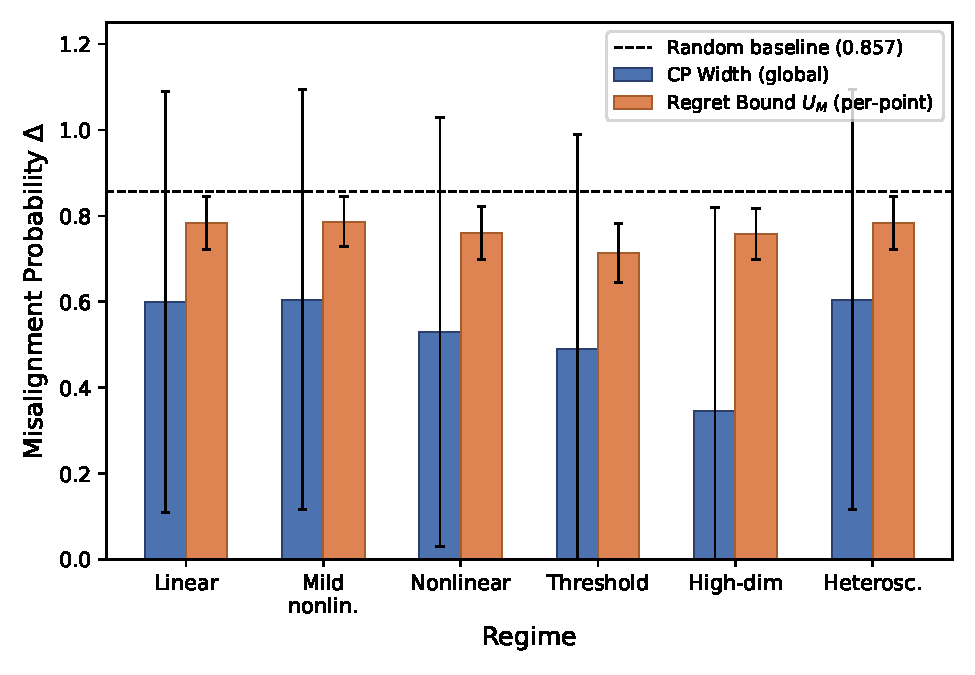
\includegraphics[width=\textwidth]{figures/figure1.pdf}
    \caption{Empirical identification of the alignment boundary between marginal CP uncertainty and conditional risk ordering. Misalignment probability $\Delta$ across six structural regimes for two surrogate functionals: global CP interval width (blue) and per-point regret bound $U_M$ (orange). The dashed line marks the random baseline ($1 - 1/7 \approx 0.857$). Error bars show $\pm 1$ standard deviation across $B = 200$ replications. Alignment is strongest in the high-dimensional regime where lasso dominates, and weakest in competitive settings (linear, heteroscedastic) where multiple estimators perform similarly. The per-point surrogate $U_M$ does not materially improve over the global surrogate, confirming that the absolute-residual quantile to L2-conditional functional gap is persistent rather than resolvable by localized smoothing in our experiments.}
    \label{fig:gap-vs-regime}
\end{figure}

\begin{figure}[t]
    \centering
    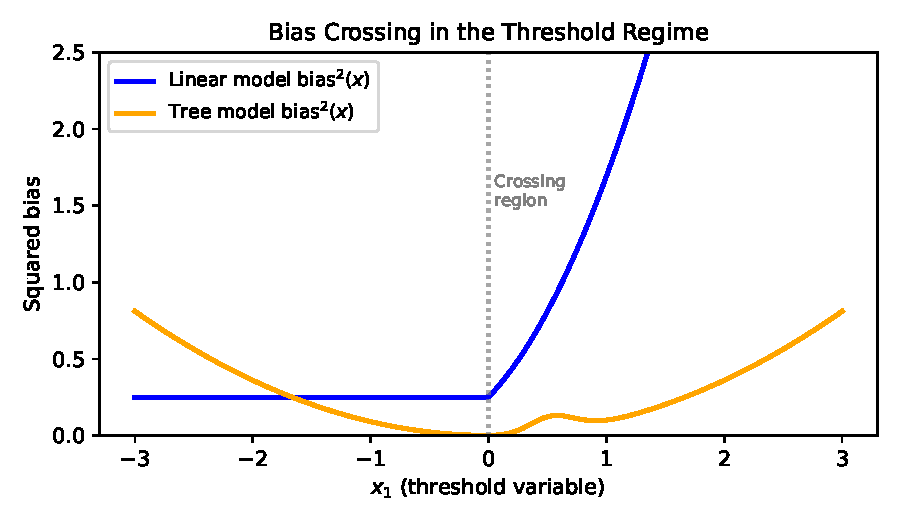
\includegraphics[width=0.7\textwidth]{figures/figure2_bias_crossing.pdf}
    \caption{Conceptual illustration of bias crossing in the threshold regime. The squared-bias functions of a linear model (blue) and a tree model (orange) cross as a function of the threshold variable $x_1$. On each side of the crossing region, a different estimator incurs lower bias; no global summary can capture this spatial reversal. This geometric mechanism is the root cause of the alignment gap under heterogeneous bias (Proposition~2).}
    \label{fig:bias-crossing}
\end{figure}

\subsection{Aggregation Inherits the Alignment Limitation}
\label{sec:aggregation}

The functional gap documented above addresses model selection: using CP signals to pick a single estimator. Does it also extend to model \textit{aggregation}? We test this using CRGA, conformalized regret-guided aggregation, which assigns per-point soft weights inversely proportional to $U_M(x)$ and re-conformalizes the fused estimator. CRGA is introduced not as a competing aggregation method but as a \textit{diagnostic intervention}: if $U_M$ captures decision-relevant uncertainty beyond what it already reveals about ranking, CRGA should outperform stacking; if the alignment limitation reflects a persistent functional gap, CRGA should inherit it.

Table~\ref{tab:aggregation} compares CRGA against equal-weight fusion and non-negative ridge stacking. The pattern is consistent: CRGA never outperforms stacking across all six regimes. The relative gap $(MSE_{\text{CRGA}} - MSE_{\text{stacking}}) / MSE_{\text{stacking}}$ ranges from +2.8\% in the linear regime to +9.2\% in the nonlinear regime. In no case does the improved ranking quality of $U_M$ translate into improved aggregation.

Tail-risk analysis reinforces this conclusion. The 95th percentile of squared error for CRGA exceeds that of stacking in all regimes, with the largest gap again in the nonlinear regime (CRGA Q95 = 7.02 versus stacking Q95 = 6.31). The conditional oracle Q95, representing the irreducible tail risk achievable if the optimal estimator were known per point, ranges from 1.09 to 2.07, far below both methods. (We note that stacking can slightly outperform the oracle in some regimes because the oracle selects a single estimator per point, whereas stacking combines multiple estimators; this is not a contradiction.)

The fact that CRGA underperforms even equal-weight fusion in the threshold and high-dimensional regimes (Table~\ref{tab:aggregation}) suggests that $U_M$-based weights are sometimes anti-correlated with estimator quality: estimators with narrow regret bounds are not necessarily better performers. This is consistent with the observation that $U_M$'s pairwise ranking accuracy, while above random, does not reliably identify the best estimator. The aggregation results confirm that the alignment limitation is decision-relevant: improved ranking of estimators does not imply improved performance in downstream tasks, whether selection or aggregation. We note that the $\Delta$ metric captures the frequency of misselection but not its severity. The top-1 regret (MSE of the CP-selected model minus the oracle MSE) is near zero across all six regimes when evaluated in expectation, because the model with the narrowest CP interval tends to have close-to-optimal average MSE even when it is not conditionally optimal at every point. This confirms that the alignment gap is about per-point decision resolution rather than global model quality. The aggregation results in Table~\ref{tab:aggregation} provide further evidence on the practical cost: when CP-width-based selection selects a suboptimal model, the MSE gap relative to the true conditional oracle is bounded in most settings (e.g., CRGA vs.\ stacking relative gap of 2.8--9.2\%).

\begin{table}[t]
    \centering
    \caption{Aggregation MSE across regimes. Oracle column shows the best single-model MSE per regime.}
    \label{tab:aggregation}
    \begin{tabular}{lcccc}
        \toprule
        Regime & Equal-Wt & Stacking & CRGA & Oracle \\
        \midrule
        Linear       & 1.210 & 1.076 & 1.106 & 1.049 \\
        Mild nonlin.   & 1.178 & 1.059 & 1.085 & 1.036 \\
        Nonlinear    & 1.882 & 1.644 & 1.795 & 1.717 \\
        Threshold    & 1.257 & 1.164 & 1.234 & 1.146 \\
        High-dim     & 1.547 & 1.415 & 1.460 & 1.429 \\
        Heterosc.    & 1.127 & 1.002 & 1.029 & 0.966 \\
        \bottomrule
    \end{tabular}
\end{table}

\subsection{Real-Data Robustness}
\label{sec:real-data}

We evaluate whether the functional gap generalizes to three publicly available datasets spanning classification and regression tasks: Home Credit Default Risk (307,511 observations, 66 features), PIMA Diabetes (768, 8), and Superconductivity (21,263, 81). We emphasize that these experiments are not intended as a benchmark comparison; the goal is to test whether the misalignment observed in controlled simulation extends to unknown, non-simulated DGPs. Unlike the simulation setting where $f_0$ is known and the conditional risk can be computed exactly, real data admits no such oracle. We therefore use test-set MSE as a high-fidelity surrogate oracle: it is an unbiased estimate of the expected generalization error and, with sufficiently many test points, approximates the integrated conditional risk. However, the resulting $\hat{\Delta}$ estimates must be interpreted with caution: they compare one marginal summary (CP width) against another (test MSE), and thus test a weaker proposition than the simulation's comparison against true conditional risk.

For each dataset, we compute $\hat{\Delta}$ across multiple random train-test splits. As shown in Table~\ref{tab:real}, the misalignment pattern varies predictably with dataset structure. On Home Credit, the CP-width-based selection is always wrong ($\hat{\Delta} = 1.00$): linear models produce narrower prediction intervals, but tree-based models achieve lower test MSE. While $\hat{\Delta} = 1.00$ may appear to suggest that CP signals are completely uninformative, this extreme result is itself consistent with the paper's core argument: the Home Credit data exhibit highly heterogeneous bias structure across a large, high-dimensional feature space, precisely the setting where Proposition~2 predicts maximal misalignment. The failure is not in the CP signal itself but in applying a marginal summary to a decision problem that requires conditional resolution. On PIMA, the misalignment is similarly high ($\hat{\Delta} = 0.82$). In contrast, on the Superconductivity dataset, where tree ensembles dramatically outperform linear methods (MSE 91 versus 311), the CP width correctly identifies the superior model class ($\hat{\Delta} = 0.00$). This variation is consistent with the boundary condition identified in Section~\ref{sec:boundary}: CP-based selection works when one estimator class dominates the others, but fails in more competitive settings.

\begin{table}[t]
    \centering
    \caption{Real-data misalignment $\hat{\Delta}$ across random train-test splits.}
    \label{tab:real}
    \begin{tabular}{lcccc}
        \toprule
        Dataset & Splits & $\hat{\Delta}$ (Width) & 95\% CI & Best Model \\
        \midrule
        PIMA            & 50 & 0.82 & [0.71, 0.93] & RF \\
        Home Credit     & 20 & 1.00 & [0.85, 1.00] & RF \\
        Supercond.      & 30 & 0.00 & [0.00, 0.10] & XGBoost \\
        \bottomrule
    \end{tabular}
\end{table}

\subsection*{Limitations and Practical Guidance}
Several limitations of this study should be noted. First, all simulations use Gaussian predictors with independent coordinates; correlated designs may produce different bias-crossing patterns. Second, the estimators use fixed hyperparameters across regimes; per-DGP tuning could shift the alignment boundary. Third, the high-dimensional regime ($p/n = 0.2$) is moderate; the alignment gap may widen or narrow at higher dimensions. Fourth, the real-data analysis compares CP width against test MSE (both marginal) and thus tests a weaker proposition than the simulation. Fifth, the CQR experiment demonstrates the difficulty of per-point adaptation under limited data but does not exhaust all possible CP variants.

For practitioners, our findings suggest a simple heuristic: CP-based model selection can be trusted when the test-bed includes a clearly dominant estimator (as in the Superconductivity dataset) but should be avoided in competitive settings with heterogeneous estimator biases. Validation-MSE or cross-validated selection provides a more reliable alternative in such settings, though it too is subject to alignment limitations under strong nonlinearity. We caution against using CP interval width as a general-purpose model selection criterion without domain-specific validation.

On the positive side, CP width can serve as a useful rapid screening tool when computational constraints prevent full cross-validation, for instance when choosing among a small number of structurally dissimilar model families (e.g., linear vs.\ tree ensembles vs.\ neural networks), where the performance gap tends to be large enough that the CP signal's ordering is reliable. The linear and threshold regimes in our study (where CP width achieves 40--51\% accuracy against a 14\% random baseline) suggest that the signal has genuine value in settings where estimator biases are approximately uniformly ordered. The key is to recognize when one is inside versus outside the alignment boundary: CP-based selection is most trustworthy when the estimator class exhibits variance-dominated risk with similar bias geometry, and least trustworthy when bias structures are heterogeneous and crossing.

% ============================================================
\section{Conclusion}
\label{sec:conclusion}
% ============================================================

This paper characterizes a persistent gap between marginal residual functionals and conditional decision risk under heterogeneous bias geometry. Conformal prediction provides valid distribution-free uncertainty intervals, but its ranking functional, whether global interval width or per-point regret bounds, operates on the absolute-residual quantile scale and marginalizes over the predictor space. Decision-optimal model selection, by contrast, requires conditional assessments of bias--variance tradeoffs at each test point. The decomposition identity (\eqref{eq:cp-decomp}--\eqref{eq:risk-decomp}) shows that these two functionals differ in aggregation (marginal versus conditional), loss scale (absolute quantile versus squared), and information structure (one scalar per estimator versus one function over $x$). Under variance-dominated conditions with uniformly ordered bias across all candidate estimators, these differences are harmless and rankings align. However, as the linear regime demonstrates (where tree-based and neural network estimators introduce approximation bias even for linear targets), the practical scope of these conditions is narrower than a theoretical taxonomy might suggest. When estimator competition is high or bias surfaces are heterogeneous, the functional gap widens and the marginal CP signal collapses the conditional risk surface, unable to resolve the spatial crossing of estimator bias profiles.

The evidence across six regimes, seven estimators, and two CP signal variants supports this characterization. Per-point misalignment probabilities approach the random baseline in all regimes with bias heterogeneity (0.71--0.79), and aggregation inherits the same limitation.

These findings characterize an alignment boundary separating regimes where marginal residual functionals are more decision-consistent from regimes where conditional risk geometry is not recoverable from any marginal summary. This boundary is governed by bias dominance and bias crossing, and plausibly extends to selection rules based on marginal summaries of residuals. On the positive side, within the class of variance-dominated, uniformly ordered bias families, the marginal ranking is more decision-consistent. The high-dimensional regime exemplifies this: lasso's dominance produces $\Delta = 0.345$, the lowest across all settings. However, the linear regime demonstrates an important caveat: even when theory predicts alignment, practical estimator diversity (tree-based and neural network approximations) can introduce sufficient bias variation to raise $\Delta$ to 0.600. The surrogate approach is therefore not universally flawed but is restricted to regimes where the conditional risk geometry is sufficiently simple and estimator competition is limited.

We emphasize that the objective of this paper is not to propose an alternative model selection procedure, but to characterize a persistent limitation of marginal residual summaries in representing conditional decision geometry. The results therefore delineate an applicability boundary rather than a failure of any specific method. Future work should explore whether alternative uncertainty quantifiers, such as full predictive distributions, quantile regression, or directly conditional risk estimators, can narrow this functional gap. Investigation of the alignment boundary in settings beyond regression, including classification and structured prediction, is also warranted.

%% ============================================================
\bibliography{refs}
%% ============================================================

\end{document}
